
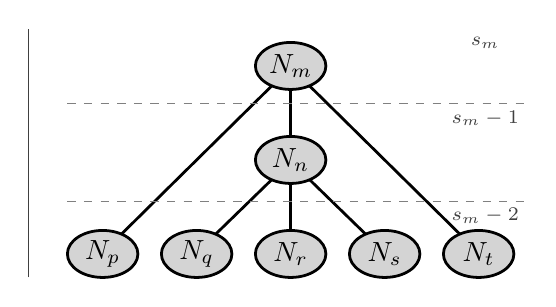
\begin{tikzpicture}[>=latex,line join=bevel,scale=0.47]
  \pgfsetlinewidth{1bp}
%%
\begin{scope}
  \pgfsetstrokecolor{black}
  \definecolor{strokecol}{rgb}{1.0,1.0,1.0};
  \pgfsetstrokecolor{strokecol}
  \definecolor{fillcol}{rgb}{1.0,1.0,1.0};
  \pgfsetfillcolor{fillcol}
  \filldraw (0bp,0bp) -- (0bp,180bp) -- (342bp,180bp) -- (342bp,0bp) -- cycle;
\end{scope}
  \pgfsetcolor{black}
  % Edge: c2 -> c6
  \draw [-] (156.43bp,74.834bp) .. controls (146.25bp,64.938bp) and (132.48bp,51.546bp)  .. (113.8bp,33.385bp);
  % Edge: root -> c4
  \draw [-] (156.4bp,146.6bp) .. controls (131.06bp,121.62bp) and (78.82bp,70.101bp)  .. (41.639bp,33.435bp);
  % Edge: c2 -> c8
  \draw [-] (185.57bp,74.834bp) .. controls (195.75bp,64.938bp) and (209.52bp,51.546bp)  .. (228.2bp,33.385bp);
  % Edge: root -> c10
  \draw [-] (185.6bp,146.6bp) .. controls (210.94bp,121.62bp) and (263.18bp,70.101bp)  .. (300.36bp,33.435bp);
  % Edge: root -> c2
  \draw [-] (171bp,143.7bp) .. controls (171bp,135.98bp) and (171bp,126.71bp)  .. (171bp,108.1bp);
  % Edge: c2 -> c7
  \draw [-] (171bp,71.697bp) .. controls (171bp,63.983bp) and (171bp,54.712bp)  .. (171bp,36.104bp);
  % Node: c7
\begin{scope}
  \definecolor{strokecol}{rgb}{0.0,0.0,0.0};
  \pgfsetstrokecolor{strokecol}
  \definecolor{fillcol}{rgb}{0.83,0.83,0.83};
  \pgfsetfillcolor{fillcol}
  \filldraw [opacity=1] (171bp,18bp) ellipse (27bp and 18bp);
  \draw (171bp,18bp) node {$\mathscr{N}_r$};
\end{scope}
  % Node: c8
\begin{scope}
  \definecolor{strokecol}{rgb}{0.0,0.0,0.0};
  \pgfsetstrokecolor{strokecol}
  \definecolor{fillcol}{rgb}{0.83,0.83,0.83};
  \pgfsetfillcolor{fillcol}
  \filldraw [opacity=1] (243bp,18bp) ellipse (27bp and 18bp);
  \draw (243bp,18bp) node {$\mathscr{N}_s$};
\end{scope}
  % Node: c2
\begin{scope}
  \definecolor{strokecol}{rgb}{0.0,0.0,0.0};
  \pgfsetstrokecolor{strokecol}
  \definecolor{fillcol}{rgb}{0.83,0.83,0.83};
  \pgfsetfillcolor{fillcol}
  \filldraw [opacity=1] (171bp,90bp) ellipse (27bp and 18bp);
  \draw (171bp,90bp) node {$\mathscr{N}_n$};
\end{scope}
  % Node: c10
\begin{scope}
  \definecolor{strokecol}{rgb}{0.0,0.0,0.0};
  \pgfsetstrokecolor{strokecol}
  \definecolor{fillcol}{rgb}{0.83,0.83,0.83};
  \pgfsetfillcolor{fillcol}
  \filldraw [opacity=1] (315bp,18bp) ellipse (27bp and 18bp);
  \draw (315bp,18bp) node {$\mathscr{N}_t$};
\end{scope}
  % Node: root
\begin{scope}
  \definecolor{strokecol}{rgb}{0.0,0.0,0.0};
  \pgfsetstrokecolor{strokecol}
  \definecolor{fillcol}{rgb}{0.83,0.83,0.83};
  \pgfsetfillcolor{fillcol}
  \filldraw [opacity=1] (171bp,162bp) ellipse (27bp and 18bp);
  \draw (171bp,162bp) node {$\mathscr{N}_m$};
\end{scope}
  % Node: c6
\begin{scope}
  \definecolor{strokecol}{rgb}{0.0,0.0,0.0};
  \pgfsetstrokecolor{strokecol}
  \definecolor{fillcol}{rgb}{0.83,0.83,0.83};
  \pgfsetfillcolor{fillcol}
  \filldraw [opacity=1] (99bp,18bp) ellipse (27bp and 18bp);
  \draw (99bp,18bp) node {$\mathscr{N}_q$};
\end{scope}
  % Node: c4
\begin{scope}
  \definecolor{strokecol}{rgb}{0.0,0.0,0.0};
  \pgfsetstrokecolor{strokecol}
  \definecolor{fillcol}{rgb}{0.83,0.83,0.83};
  \pgfsetfillcolor{fillcol}
  \filldraw [opacity=1] (27bp,18bp) ellipse (27bp and 18bp);
  \draw (27bp,18bp) node {$\mathscr{N}_p$};
\end{scope}
%
\draw[darkgray, thin] (-30bp,0bp) -- (-30bp,190bp);
\draw[gray,thin,dashed] (0bp,58bp) -- (350bp,58bp);
\draw[gray,thin,dashed] (0bp,133bp) -- (350bp,133bp);

\draw (320bp,180bp) node[darkgray] {\scriptsize $s_m$};
\draw (320bp,122bp) node[darkgray] {\scriptsize $s_m - 1$};
\draw (320bp,47bp) node[darkgray] {\scriptsize $s_m - 2$};
\end{tikzpicture}

